\documentclass[a4paper,12pt, oneside]{book}

%\usepackage{fullpage}
\usepackage[italian]{babel}
\usepackage[utf8]{inputenc}
\usepackage{amssymb}
\usepackage{amsthm}
\usepackage{graphics}
\usepackage{amsfonts}
\usepackage{listings}
\usepackage{amsmath}
\usepackage{amstext}
\usepackage{engrec}
\usepackage{rotating}
\usepackage[safe,extra]{tipa}
\usepackage{showkeys}
\usepackage{multirow}
\usepackage{hyperref}
\usepackage{microtype}
\usepackage{enumerate}
\usepackage{braket}
\usepackage{marginnote}
\usepackage{pgfplots}
\usepackage{cancel}
\usepackage{polynom}
\usepackage{booktabs}
\usepackage{enumitem}
\usepackage{framed}
\usepackage{pdfpages}
\usepackage{pgfplots}
\usepackage[cache=false]{minted}
\usepackage{fancyhdr}
\pagestyle{fancy}
\fancyhead[LE,RO]{\slshape \rightmark}
\fancyhead[LO,RE]{\slshape \leftmark}
\fancyfoot[C]{\thepage}



\title{Sistemi distribuiti}
\author{UniShare\\\\Davide Cozzi\\\href{https://t.me/dlcgold}{@dlcgold}\\\\Gabriele De Rosa\\\href{https://t.me/derogab}{@derogab} \\\\Federica Di Lauro\\\href{https://t.me/f_dila}{@f\textunderscore dila}}
\date{}

\pgfplotsset{compat=1.13}
\begin{document}
\maketitle

\definecolor{shadecolor}{gray}{0.80}

\newtheorem{teorema}{Teorema}
\newtheorem{definizione}{Definizione}
\newtheorem{esempio}{Esempio}
\newtheorem{corollario}{Corollario}
\newtheorem{lemma}{Lemma}
\newtheorem{osservazione}{Osservazione}
\newtheorem{nota}{Nota}
\newtheorem{esercizio}{Esercizio}
\tableofcontents
\renewcommand{\chaptermark}[1]{%
\markboth{\chaptername
\ \thechapter.\ #1}{}}
\renewcommand{\sectionmark}[1]{\markright{\thesection.\ #1}}
\chapter{Introduzione}
\textbf{Questi appunti sono presi a le lezioni. Per quanto sia stata fatta una revisione è altamente probabile (praticamente certo) che possano contenere errori, sia di stampa che di vero e proprio contenuto. Per eventuali proposte di correzione effettuare una pull request. Link: } \url{https://github.com/dlcgold/Appunti}.\\
\textbf{Grazie mille e buono studio!}
\chapter{Lezione 1}
\textit{Un sistema distribuito è un sistema nel quale componenti hardware e software, collocati in computer connessi alla rete, comunicano e coordinano le loro azione solitamente col passaggio di messaggi (a differenza delle chiamate di procedura che si hanno col passaggio di parametri su memoria condivisa)}. Ogni processo ha quindi una parte di logica applicativa e una parte di coordinamento. Altrimenti si ha questa definizione. \textit{un sistema distribuito è un insieme di elementi autonomi di computazione che si interfacciano agli utenti come un singolo sistema "coerente"}.
\begin{center}
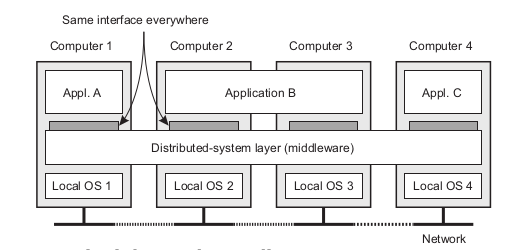
\includegraphics[scale=2.5]{img/cli.png}
\end{center}
I sistemi distribuiti sono quindi sistemi complessi. Si hanno le seguenti caratteristiche:
\begin{itemize}
\item le unità autonome di computazione si chiamano \textbf{nodi} e possono essere device hardware o singoli processi software
\item ogni nodo "fa quello che vuole", ogni nodo è autonomo, e vanno tra loro sincronizzati e coordinati (programmazione concorrente). Ogni nodo ha la sua "nozione di tempo"
\item utenti e applicazioni vedono un singolo sistema
\item si possono aprire e chiudere gruppi di nodi
\end{itemize}
La parola chiave è \textbf{trasparenza di distribuzione (distribution trasparency)}. Trasparenza significa nascondere dettagli agli utenti che possono ignorare ciò che succede e che non possono modificare il servizio. Si ha che il sistema non va in errore se un solo nodo va in errore in quanto i nodi sono indipendenti ma è difficile occultare gli errori parziali dei singoli nodi ed è difficile sistemare gli eventuali errori del singolo nodo. Ovviamente non si ha memoria condivisa e non c'è uno stato globale. In un sistema distribuito non si ha un clock globale e non si può controllare globalmente o avere uno scheduling globale.
\subsection{Il modello Client-Server}
\begin{center}
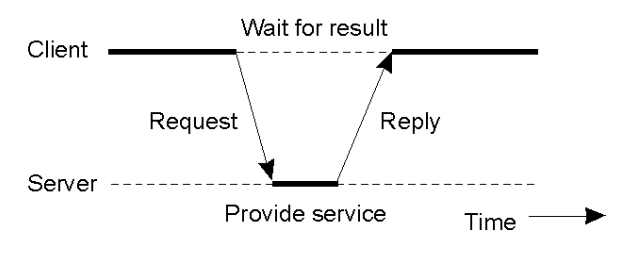
\includegraphics[scale=0.6]{img/cli2.png}
\end{center}
Si ha che un client fa una richiesta e il server risponde con un certo risultato (con il conseguente ritardo, a differenza del modello a chiamata di procedura).  
\begin{center}
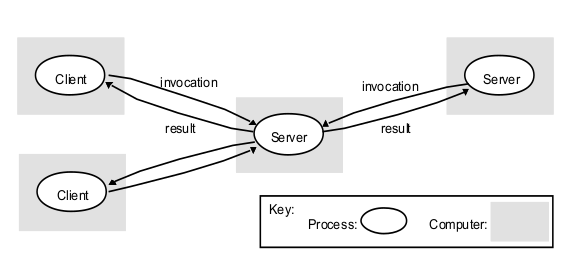
\includegraphics[scale=2.6]{img/cli3.png}
\end{center}
Si può accedere a server multipli (cluster con anche bilanciamento del carico) e si può accedere via proxy (dei server "finti" che fungono da concentratori).\\
Un sistema distribuito ha 4 problemi da fronteggiare:
\begin{enumerate}
\item \textbf{identificare la controparte}, che si risolve assegnando un nome, è la procedura di \textbf{naming}
\item \textbf{accedere alla controparte}, che si risolve con una reference, un \textbf{access point}
\item \textbf{comunicare (parte 1)}, che si risolve accettando e condividendo un formato, un \textbf{protocollo, "protocol"}
\item \textbf{comunicare (parte 2)}, che si risolve concordando \textit{sintassi e semantica} per l'informazione da condividere \textbf{(quest'ultimo è però ancora un problema aperto)}
\end{enumerate}
Si hanno le seguenti definizioni per quanto riguarda la trasparenza:
\begin{itemize}
\item \textbf{naming}, usare nomi simbolici per identificare le risorse che sono parte del sistema distribuito
\item \textbf{access trasparency}, nascondere le differenze nella rappresentazione delle informazioni e nell'accedere ad un'informazione locale o remota 
\item \textbf{location trasparency}, nascondere dove è collocata una risorsa sulla rete
\item  \textbf{relocation or mobility transparency}, nascondere che una risorsa può essere stata trasferita ad un'altra locazione mentre è in uso
\item \textbf{migration trasparency}, nascondere che una risorsa può essere trasferita
\item \textbf{replication transparency}, nascondere che una risorsa può essere replicata
\item \textbf{concurrency transparency}, nascondere che una risorsa può essere condivisa da molti utenti indipendenti
\item \textbf{failure trasparency}, nascondere fallimenti e recovery di una risorsa
\item \textbf{persistence trasparency}, nascondere se una risorsa è volatrile o memorizzata permanentemente
\end{itemize}
non si possono però nascondere:
\begin{itemize}
\item \textbf{ritardi e latenze di comunicazione}
\item \textbf{nascondere completamente i failure della rete e dei nodi}, non puoi neanche distinguere bene rallentamenti e errori. Ovviamente non puoi sapere se sta per accadere un \textbf{crash}
\end{itemize}
Una trasparenza completa, oltre ad essere quasi impossibile a livello teorico, è anche estremamente "cara" a livello di performances e tempistiche (causa scrittura costante su dischi e mantenimento delle repliche).\\
Nascondere le informazioni è alla base dell'ingegneria del software. Bisogna separare il \textit{cosa} si fa e il \textit{come} lo si fa. Il \textit{cosa} si fa mediante la definizione dell'interfaccia, \textit{Interface Definition Languages (IDL)}, e il \textit{come} mediante l'implementazione delle classi e dei metodi. Le interfacce sono definite mediante principi standard, sono complete e sono neutrali (indipendenti dall'implementazione).
\begin{center}
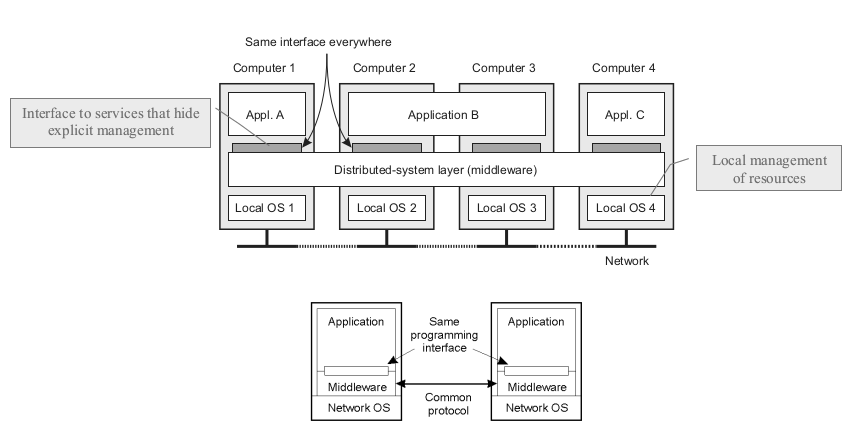
\includegraphics[scale=2]{img/cli4.png}
\end{center}
Tra i vari componenti si ha:
\begin{itemize}
\item \textbf{indipendenza logica}, con i vari componenti che lavorano autonomamente
\item \textbf{composizione}, con la collaborazione dei vari processi
\end{itemize}
Si separano:
\begin{itemize}
\item \textbf{meccanismi}, ciò che è fatto dai componenti (esempio il context switch)
\item \textbf{politiche}, come vengono applicati le varie funzionalità del sistema (esempio lo scheduling Round Robin RR)
\end{itemize}
Bisogna separare e bilanciare politiche e meccanismi
\begin{center}
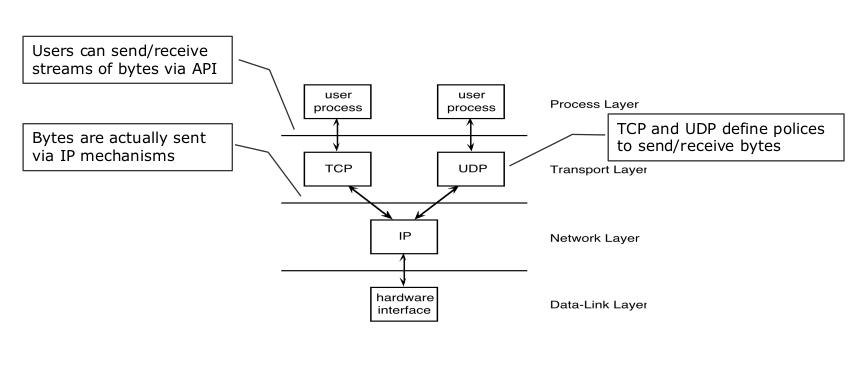
\includegraphics[scale=2]{img/cli5.png}
\end{center}
Ricapitolando il concetto di protocollo:
\begin{itemize}
\item per poter capire le richieste e formulare le risposte i due processi devono concordare un protocollo
\item i protocolli (come \textit{HTTP, FTP e SMTP}) definiscono il formato, l'ordine di invio e di ricezione dei messaggi tra i dispositivi, il tipo dei dati e le azioni da eseguire quando si riceve un messaggio
\item le applicazioni su TCP/IP:
\begin{itemize}
\item si scambiano stream di byte di lunghezza infinita (il meccanismo)
\item che possono essere segmentati in messaggi (la politica) definiti da un protocollo condiviso
\end{itemize}
\end{itemize}
Vediamo un esempio di codice. Partiamo dall'\textit{header.h}
\begin{minted}{c}
// definizioni necessarie a client e server 

#define TRUE 1
#define MAX_PATH 255 // lunghezza massima del nome di un file
#define BUF_SIZE 1024 // massima grandezza file trasferibili per volta
#define FILE_SERVER 243 // indirizzo di rete del file del server

// operazioni permesse 

#define CREATE 1 // crea un nuovo file
#define READ 2 // legge il contenuto di un file e lo restituisce
#define WRITE 3 // scrive su un file
#define DELETE 4 // cancella un file

// errori

#define OK 0 // nessun errore
#define E_BAD_OPCODE -1 // operazione sconosciuta
#define E_BAD_PARAM -2 // errore in un parametro
#define E_IO -3 // errore del disco o errore di I/O

// definizione del messaggio

struct message{
  long source; // identità del mittente
  long dest; // identità del ricevente
  long opcode; // operazione richiesta
  long count; // numero di byte da trasferire
  long offset; // posizione sul file da cui far partire l'I/O
  long result; // risultato dell'operazione
  char name[MAX_PATH]; // nome del file
  char data[BUF_SIZE]; //informazione da leggere o scrivere
};
\end{minted}
\newpage
vediamo la struttura di un semplice server che realizza un semplice file server remoto:
\begin{minted}{c}
#include <header.h>
void main(void){
  struct message m1, m2; // messaggio in entrata e uscita
  int r; // risultato
  
  while(TRUE){ // il server è sempre in esecuzione
    receive(FILE_SERVER, &m1); // stato di wait in attesa di m1
    switch(m1.code){ // vari casi in base alla richiesta
      case CREATE: 
        r = do_create(&m1, &m2);
        break;
      case CREATE: 
        r = do_read(&m1, &m2);
        break;
      case CREATE: 
        r = do_write(&m1, &m2);
        break;
      case CREATE: 
        r = do_delete(&m1, &m2);
        break;
      default:
        r = E_BAD_OPCODE;
    }
    
    m2.result = r; // ritorna il risultato al client
    send(m1.source, &m2); // manda la risposta
    
  }
}  
\end{minted}
\newpage
vediamo ora un client che usa il servizio per straferire un file:
\begin{minted}{c}
#include <header.h>

int copy(char *src, char *dst){ // copia file usando il server
  strcut message m1; // buffer del messaggio
  long position; // attuale posizione del file
  long client = 110; // indirizzo del client
  
  initialize(); // prepara l'esecuzione
  position = 0; 
  do{
    m1.opcode = READ; // operazione settata su READ
    m1.offset = position; // scelta la posizione nel file
    m1.count = BUF_SIZE; // byte da leggere
    strcpy(&m1.name, src); // nome file copiato in m1
    send(FILESERVER, &m1); // manda il messaggio al file server
    receive(client, &m1); // aspetta la risposta
    
    // scrive quanto ricevuto su un file di destinazione
    m1.opcode = WRITE; // operazione settata su WRITE
    m1.offset = position; // scelta la posizione nel file
    m1.count = BUF_SIZE; // byte da leggere
    strcpy(&m1.name, dst); // nome del file sul buffer
    send(FILESERVER, &m1); // manda il messaggio al file server
    receive(client, &m1); // aspetta la risposta
    position += m1.result // il risultato sono i byte scritti
  }while(m1.result > 0); // itera fino alla fine
  return(m1.result >= 0 ? OK : m1.result); // ritorna OK o l'errore
}

\end{minted}
\end{document}